% @author: MetaboHUB
% @date: 2014/02/27
% @note: this document is versioned through a GIT repository; sharing is caring

\documentclass[a4paper,11pt]{article}

%%%%%%%%%%%%%%%%%%%
% Polices 
\renewcommand*\sfdefault{cmss}
\renewcommand*\familydefault{\sfdefault}  %% Only if the base font of the document is to be sans serif

%%%%%%%%%%%%%%%%%%%
% packages
\usepackage{cmbright}
\usepackage{algorithm}
\usepackage{algorithmic}
\usepackage{amssymb}
\usepackage{amsmath}
\usepackage{pifont}
\usepackage[usenames,dvipsnames]{color}

\usepackage{wallpaper}
\usepackage[utf8]{inputenc} % accents
\usepackage[english]{babel}
\usepackage{fixltx2e}

\usepackage{array}
\usepackage{color}

% margins
\usepackage{geometry}
\geometry{left=2.3cm,right=2.3cm,top=3cm,bottom=2cm}

% pdf hyperlinks
\usepackage{hyperref}

%%%%%%%%%%%%%%%%%%%%%%%%%%%%%%%%%%%%%%%%%%%%%%%%%%%%%%%%%%%%%%%%%%%%% metadata

\usepackage{hyperref}
\usepackage{color}

\hypersetup{
	pdftitle={PeakForest - a spectral database - Software Requirement Specification},
	pdfauthor={MetaboHUB - WP3},
	colorlinks=true,
	urlcolor=blue,
	linkcolor=black,
	citecolor=black,
}
\usepackage{afterpage}
% dates
\usepackage{datetime}
\usepackage{multirow}
\usepackage{tabularx}
\usepackage{hyperref}
\usepackage{pifont}

% italic text
\newcommand{\ie}{\textit{i.e.}~}
\newcommand{\eg}{\textit{e.g.}~}
%\newcommand{\exp}{\textit{exp}~}
\newcommand{\cf}{\textit{cf.~}}
\newcommand{\textitt}[1]{\textit{\texttt{#1}}}
\def\myversion{0.1}

%tickmarks
\newcommand{\tick}{\textcolor{ForestGreen}{\ding{52}}}
\newcommand{\tickNo}{\hspace{1pt}\textcolor{BrickRed}{\ding{55}}}

%colors
%\usepackage[table]{xcolor}
\definecolor{inraGreen}{rgb}{0.50196078431,0.62745098039,0}
\definecolor{mthRed}{rgb}{1,0.00784313725,0.00784313725}
%%%%%%%%%%%%%%%%%%%

% meta-data
\author{MetaboHUB - WP3}
\date{2014}

%%%%%%%%%%%%%%%%%%%
% title page 
\newcommand{\HRule}{\rule{\linewidth}{0.5mm}}

% version
\input{vc.tex}

\begin{document}

%%%%%%%%%%%%%%%%%%%%%%%%%%%%%%%%%%%%%%%%%%%%%%%%%%%%%%%%%%%%%%%%%%%%% title page
% @author: MetaboHUB
% @date: 2014/02/20
% @note: this document is versioned through a GIT repository; sharing is caring

\begin{titlepage}

\begin{center}

% Upper part of the page

\includegraphics[width=0.7\textwidth]{./files/images/mth_title.jpg}\\[1cm] 

% Title
\HRule \\[0.4cm]
\begin{center} { \textsc{\large { \huge \bfseries \colorbox{Black}{\color{White}Metabo{\color{mthRed}HUB}} WP3 \\}} } \end{center} %\\[0.4cm]
\begin{center} { \textsc{\large { \huge \bfseries PeakForest}} } \end{center} %\\[0.4cm]
\begin{center} { \huge \bfseries Software Requirement Specification - v 1.0} \end{center} 

%{ \huge \bfseries }\\[0.4cm]
\HRule \\[0.4cm]

 \large A MeTaboHub spectral library web-portal dedicated to metabolomic  annotation data.

\HRule \\[1.5cm]

% Author and date
\begin{flushleft}
 \large
Leading partner: INRA, CEA, CNRS, Inserm, INSA, Universit\'e de Bordeaux, Universit\'e de Toulouse III, Universit\'e Blaise Pascal, UPMC \\[\baselineskip]
Authors: Franck Giacomoni, Nils Paulhe \\[\baselineskip]
Validator: \'Etienne Th\'evenot \\[\baselineskip]
Date: \today

% version
\let\thefootnote\relax
\footnotetext{Base revision~\GITAbrHash, \GITAuthorDate, \GITAuthorName.}

\end{flushleft}

\vfill

\end{center}

\end{titlepage}

%% version
%\let\thefootnote\relax
%\footnotetext{Base revision~\GITAbrHash, \GITAuthorDate, \GITAuthorName.}

% logo on corener
%\ULCornerWallPaper{0.30}{files/xxx.jpg}
\URCornerWallPaper{0.20}{files/images/logo_mth.png}
%%%%%%%%%%%%%%%%%%%

\tableofcontents

\listoffigures


\newpage

%%%%%%%%%%%%%%%%%%%%%%%%%%%%%%%%%%%%%%%%%%%%%%%%%%%%%%%%%%%%%%%%%%%%% START

\section{Revision History}

\begin{itemize}
	\item 2014/02/28: v 0.1: first version; build table of content.
	\item 2014/09/05: v 0.2: second version; manage organization
	\item 2015/01/22: v 0.3: current version; introduction with short description
\end{itemize} 


%%%%%%%%%%%%%%%%%%%%%%%%%%%%%%%%%%%%%%%%%%%%%%%%%%%%%%%%
%% 									INTRODUCTION
%%%%%%%%%%%%%%%%%%%%%%%%%%%%%%%%%%%%%%%%%%%%%%%%%%%%%%%%

\section{Introduction}

% see : http://en.wikipedia.org/wiki/Software_requirements_specification
\subsection{Aims of the document}

This document is a support to:
\begin{itemize}
	\item list clearly objectives of the present project
	\item facilitate exchanges and communication between final users and the development team on specifications, requirement and vocabularies ;
	\item list all the requirements by software designing, development and testing.
	\item present concepts, mock up and managing processes of the spectral database.
\end{itemize} 

\subsection{Short project presentation}
\hspace*{\parindent}
This project describe the software framework development (web portal, database and tools) to provide a centralized spectral library  and annotation spectral tools for the The French National infrastructure for metabolomics and fluxomics (METABOHUB).

The principal motivation is based on open data concept and knowledge sharing inside the consortium.

There is no existing solution in any MetaboHub (MTH) team. Only emerging public repositories like {\color{red} MetaboLight, USA?, Mery-b [ref??]} today's existing. They allow to store, define and gather metabolomics data but without tools to query/enrich them. All MetaboHub laboratories store their spectral annotation on different  electronic formats.

Resources are assigned on the data model design, the web application building and data collecting templates. This work will permit for final users data browsing, searching, centralizing and annotating.

This project is leaded by Franck Giacomoni, Biological Computing Ingenior in Metabolomics at Human Nutrition Unit, INRA, Clermont Ferrand. The developing part is carried out by Nils Paulhe, in charge of the PeakForest API, Daniel Jacob and Marie Lebfevre for NMR tools and Pierrick Roger-Mele, Etienne Thevenot for MS tools.

No external prestation is required.

\subsection{Objectives}
\hspace*{\parindent}
In the context of the MetaboHUB infrastructure, the work package 3 and its task 3.6 has the aims to provide a spectral database. This work is based on the following main objectives:
\begin{itemize}
	\item Provides an online centralised resource that must help in identification : From a processed peak table (MS / NMR) and from a raw fingerprint (MS/MS, 1D NMR, 2D NMR …)
	\item Aggregating lab knowledge around metabolomic data : gathering and sharing  compounds, spectra, analytical metadata from all MTH consortium members
\end{itemize}

\subsection{Definitions}

This document use concept and definition described in wikipedia \footnote{source: \url{http://en.wikipedia.org/wiki/}},  which help us to present technical terms in an simple way for each collaborator of this document.

\begin{description}
	\item [Web-portal:] Web pages which gather information from diverse sources.
	\item [GUI (computing):] Graphical User Interface - allows users to interact with the software through graphical icons and visual indicators.
	\item [Database (computing):] Organized collection of data in a way that supports processes requiring this information.
	\item [Library (computing):] Collection of implementations of behavior, written in terms of a language, that has a well-defined interface by which the behavior is invoked.
	\item [Security (computing / networking):] Processes and mechanisms deployed to protect the data from unintended or unauthorized access.
	\item [API (computing):] Application programming interface - interface specifies how some software components should interact with each other.
	\item [Web services or WS:] Method of communication between two electronic devices over World Wide Web.
	\item [REST:] Representational State Transfer - Standard used to exchange data between computer using internet technologies.
	\item [SOAP:] Simple Object Access Protocol - Protocol specification for exchanging structured information in the implementation of web services.
	\item [UML:] Unified Modeling Language - General-purpose modeling language in the field of software engineering designed to provide a standard way to visualize the design of a system
\end{description}


%\subsubsection{Tasks}
%\begin{itemize}
%	\item Building a "Spectral Libraries Management System" (chemical library / spectral collection provided by the consortium partners).
%	\item Development and implementation of algorithms for the peak matching process.
%	\item Implementation of a decision tree for the identification process, based on priority, relevance and quality of each spectra library including the available public ones.
%	\item An "annotation framework" based on user expertise and using public resources (banks, ontology, …)
%\end{itemize}

%\subsection{System overview}

%%%%%%%%%%%%%%%%%%%%%%%%%%%%%%%%%%%%%%%%%%%%%%%%%%%%%%%%
%% 									APPLICATIVES SPEC
%%%%%%%%%%%%%%%%%%%%%%%%%%%%%%%%%%%%%%%%%%%%%%%%%%%%%%%%

\section{Applicative specifications}

\subsection{Proposed Services}

The software will provide the following services:
\begin{itemize}
	\item a tool to add referenced Chemical Compound from users chemical libraries.
	\item a tool to add spectral analysis data (NMR, MS and MSMS sources).
	\item an annotation tool for spectral analysis data.
	\item an access to a pool of public / private spectral banks (HMDB, KEGG, MassBank, PhytoHub, MeryB) 
	\item a tool to compare spectral analysis.
	\item a search engine to exploit spectral data stored in the database.
	\item a tool to aggregate data from different databases on a specific pattern (\eg source: human / plasma ...)
\end{itemize}

\begin{figure}[htbp]
	\centering
	\fbox{
		\begin{minipage}{17 cm}
			\centering
			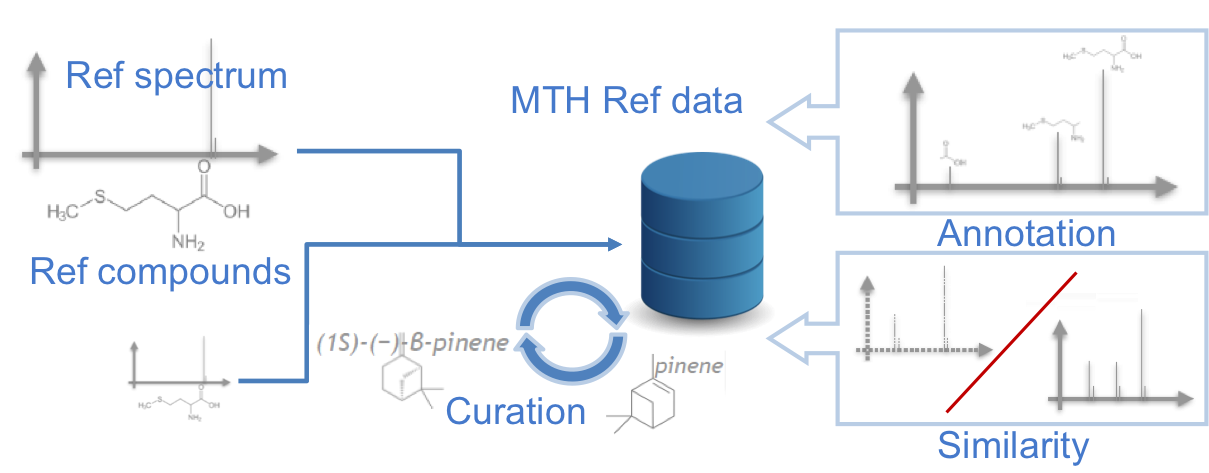
\includegraphics[height=.26\textheight,page=1]{files/images/peakforest_services.png}
			\caption{PeakForest services}
			\label{PeakForestServices}
		\end{minipage}
	}
\end{figure}


\subsection{Interface contents}
\hspace*{\parindent}
The main page proposes a global search area on the database and specific functionalities are available after user login.
We do the choice of a simple and ergonomic web interface. Most of properties or functionalities use a small number of pages.

The web portal will be design as describe in the following figure :

\begin{figure}[htbp]
	\centering
	\fbox{
		\begin{minipage}{17 cm}
			\centering
			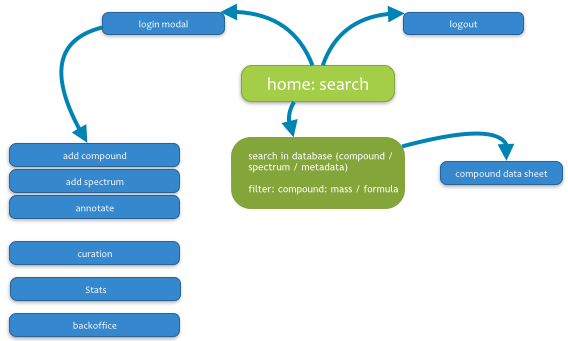
\includegraphics[height=.40\textheight,page=1]{files/images/peakforest_sitemap.png}
			\caption{PeakForest Site map}
			\label{PeakForestSiteMap}
		\end{minipage}
	}
\end{figure}


The PeakForest is built into two parts : the public user part and the administrator part. The different roles available on PeakForest are describe in a next section.

The following array present the list and features of future screens. This array present a list a global functions proposed by the interface. In its final version, PeakForest won't provide each functionality on a distinct web page. Some of them can be merge or available by a tab or a button for example.

\begin{table}[h]
	\centering
	\begin{tabular}{|c|c|c|}
		\cline{1-3}
		\textbf{Page name}   	& 	\textbf{Function}              			& 	\textbf{Data object}		\\ \cline{1-3}
		\textit{home}       		& 	Global search                  			& 	All                  			\\ \cline{1-3}
		\textit{addcompound} 	& 	Add, merge a chemical compound 	&	Compound            		\\ \cline{1-3}
		\textit{addspectrum} 		& 	Add, merge a spectrum          		& 	Spectrum             		\\ \cline{1-3}
		\textit{addcompounds} 	& 	Add, merge a list of compounds 	&	Compound            		\\ \cline{1-3}
		\textit{addspectra} 		& 	Add, merge a list of spectra      		& 	Spectrum             		\\ \cline{1-3}
		\textit{compoundidcard} 		& 	show compound features          	& 	Compound             		\\ \cline{1-3}
		\textit{editcompound} 	& 	Edit a chemical compound 		&	Compound            		\\ \cline{1-3}
		\textit{spectrumlidcard} 		& 	show spectrum features          	& 	Spectrum             		\\ \cline{1-3}
		\textit{editspectrum} 		& 	Edit a spectrum	          		& 	Spectrum             		\\ \cline{1-3}
		\textit{backoffice} 		& 	manage logins and roles           	& 	User		             		\\ \cline{1-3}
		\textit{TODO} 			& 	          						& 			             		\\ \cline{1-3}
	\end{tabular}
\end{table}


\subsection{Users}

PeakForest is designed for \textbf{chemists} and scientists using Metabolomics as an approach in their studies. A chemist will add, merge, edit, view, query data like compounds and spectra. A group of chemists (\textbf{curator}) will be in charge of the database contents quality by editing, fixing compounds and spectra features.
This information system provides also tools and interface necessary for \textbf{bioinformaticians} to facilitate massive data import/export, queries in a batch mode and ensure interoperability with others external applications.


\subsection{Users/Interface interaction}

Through PeakForest interfaces, a user should:
\begin{itemize}
	\item import a chemical compound and/or a spectrum (MS or NMR)
	\item update 1 or N compounds and 1 or N spectra
	\item search in the spectral library
	\item match experimental data against NMR  or MS/MS libraries
	\item fix errors or complete missing data for chemical compound and spectra
\end{itemize}

We established a model for users-interfaces interactions with the following UML diagram examples. Others diagrams are available in the appendix part of this document.

\begin{figure}[h!]
	\centering
	\fbox{
	\begin{minipage}[b]{0.4\linewidth}
		\centering
		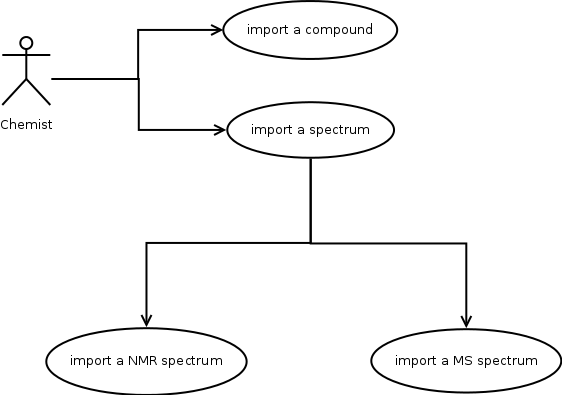
\includegraphics[height=.14\textheight]{files/images/peakforest_gui_uml_import.png}
		\caption{A chemist imports a compound and/or a spectrum.} 
		\label{GuiUmlChemistImport}
	\end{minipage}
	}
	\quad
	\fbox{
	\begin{minipage}[b]{0.4\linewidth}
		\centering
		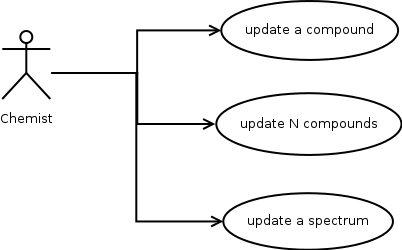
\includegraphics[height=.14\textheight]{files/images/peakforest_gui_uml_update.png}
		\caption{A chemist updates 1 or N compounds and 1 or N spectra.}
		\label{GuiUmlChemistUpdate}
	\end{minipage}
	}
\end{figure}

\subsection{Database contents}

With a model-view-controler software architectural pattern, the database structure is linked with the data model design.
The data model will integrate the following objects:
\begin{itemize}
	\item chemical compound
	\item spectral
	\item metadata
	\item users
\end{itemize}

The view of the data model is available in appendix \ref{AppendixDataModel} and each object is defined in next sub-section of the document.

\subsubsection{A compound}
\hspace*{\parindent}
A compound object is defined as the representation of a chemical entity. This entity is a chemical compound with properties such as 2d or 3d structure, molecular weight or cross references in public databases (external links like ID). This object is complex and has different levels and features. The following figure resumes this point :
	
\begin{figure}[htbp]
	\centering
	\fbox{
		\begin{minipage}{16 cm}
			\centering
			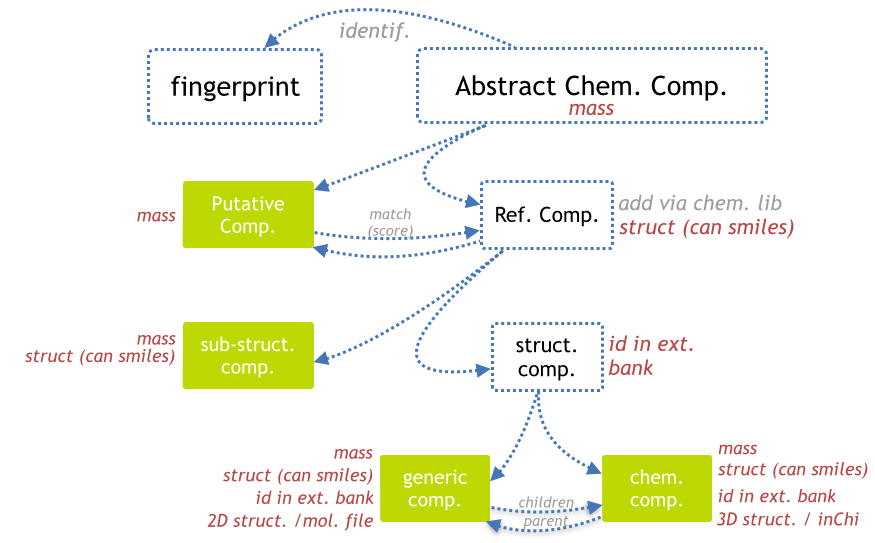
\includegraphics[height=.40\textheight,page=1]{files/images/peakforest_compound_matryoshkadoll.png}
			\caption{PeakForest -  The matryoshka doll compound object }
			\label{PeakForestCompoundObject}
		\end{minipage}
	}
\end{figure}

We dissociate several compound cases defined as standards, fragments, sub-structures, generic compounds and unknowns. These cases aims to cover all forms observed in signal annotation steps.


\subsubsection{A spectrum}

A spectrum object is defined as the representation of a analytical entity. The fingerprint comes from a mass spectrometer, a nuclear magnetic resonance spectrometer coupled with different tools such as chromatography (liquid or gas). 

\hspace*{\parindent}
According liquid chromatography - mass spectrometry conditions, we obtained for a sample a fingerprint  as a three-dimensional vector with retention time, exact mass and intensity. The retention time and the exact mass characterize the ions present in the sample and the intensity is proportional to the amount of these ions in this sample. For a classical LC-MS analysis, in one sample, from 5 to 10 thousands of ions are detected.

These data can also be graphically represented by:

\begin{itemize}
	\item a 3D-map which represents in a 3D-view the vector (retention time, exact-mass, intensity),
	\item a  Total Ion Chromatogram or TIC which represents the vector (retention time, sum(intensities)),
	\item a  Extracted Ion Chromatogram or EIC, which represents a vector (retention time, intensity) for a particular exact mass or a spectrum which represents a vector (exact mass, intensity) for a particular retention time
\end{itemize}

The following figures show examples of graphical representations.

%%%% Grapical Examples of LCMS signals

\begin{figure}[h!]
	\centering
	\fbox{
	\begin{minipage}[b]{0.25\linewidth}
		\centering
		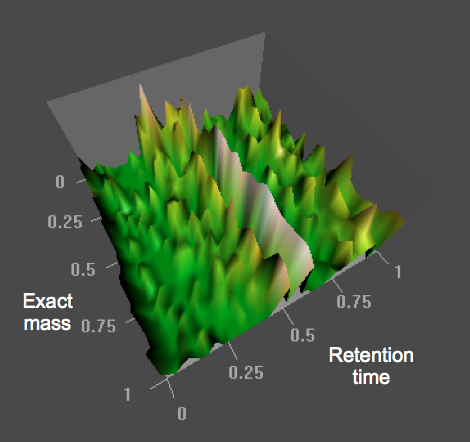
\includegraphics[height=.11\textheight]{files/images/spectrum_3d_map_example.png}
		\caption{A 3D-map spectral representation} 
		\label{Spectral3DMapRepresentation}
	\end{minipage}
	}
	\quad
	\fbox{
	\begin{minipage}[b]{0.60\linewidth}
		\centering
		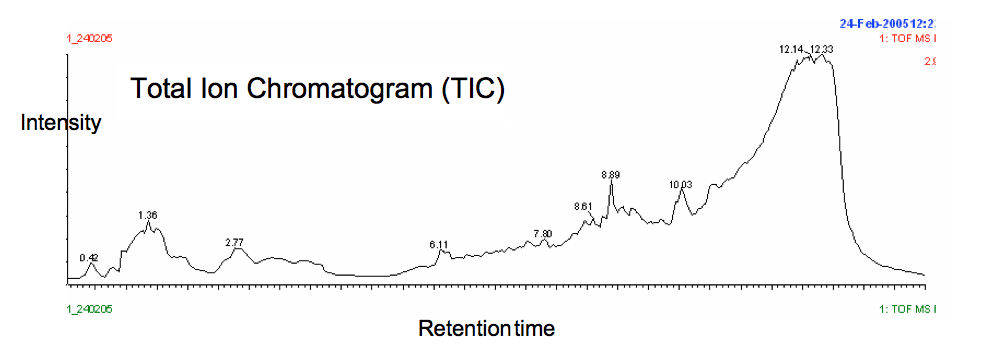
\includegraphics[height=.13\textheight]{files/images/spectrum_tic_example.png}
		\caption{Example of a TIC representation}
		\label{SpectralTICRepresentation}
	\end{minipage}
	}
\end{figure}


\begin{figure}[htbp]
	\centering
	\fbox{
	\begin{minipage}[b]{0.45\linewidth}
		\centering
		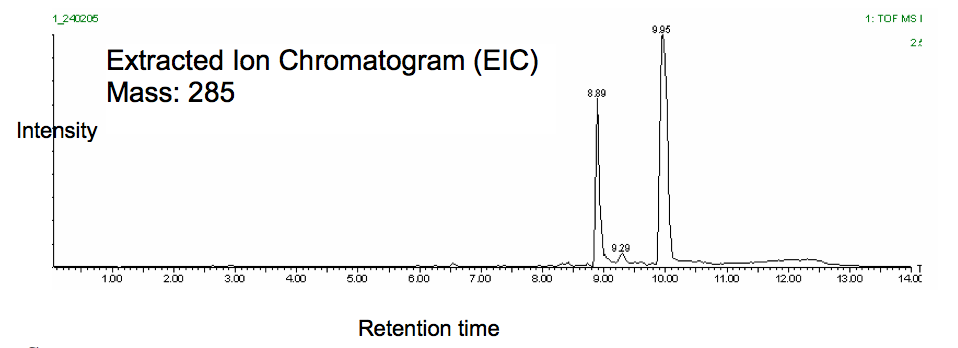
\includegraphics[height=.11\textheight]{files/images/spectrum_eic_example.png}
		\caption{Example of a EIC spectral representation}
		\label{SpectralEICRepresentation}
	\end{minipage}
	}
	\quad
	\fbox{
	\begin{minipage}[b]{0.40\linewidth}
		\centering
		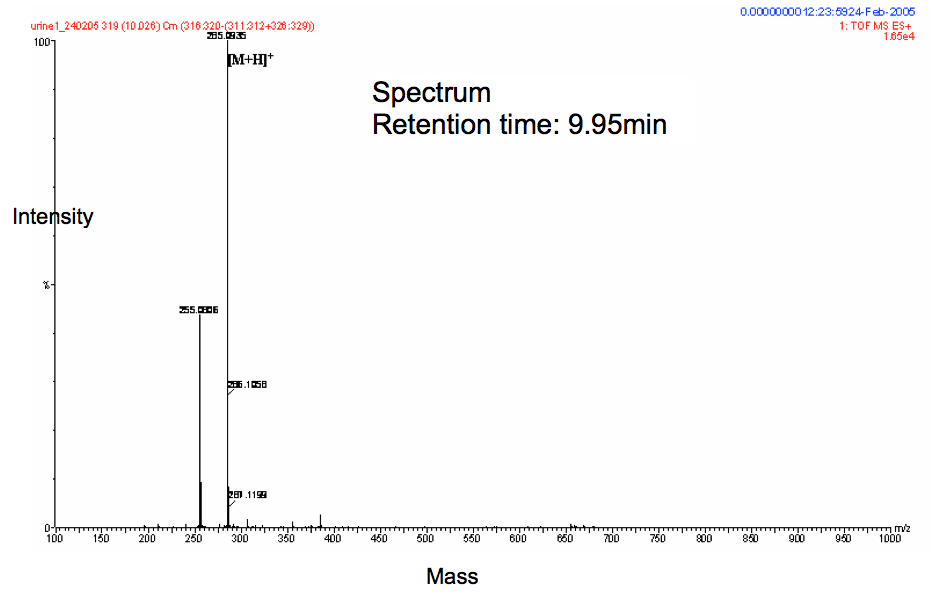
\includegraphics[height=.11\textheight]{files/images/spectrum_example.png}
		\caption{Example of a spectrum representation}
		\label{SpectrumRepresentation}
	\end{minipage}
	}
\end{figure}

%%%% Grapical Examples of GCMS signals
In gas-chromatography conditions, mass spectrometer produce same type of signals that is described below.\\


%%%% Grapical Examples of NMR signals
With nuclear magnetic resonance spectrometer, the signal is represented by different ways. The raw form or free induction decay (FID) is the nuclear magnetic resonance response obtained by excitation of the sample with radio frequency pulse. A Fourier transform is done to extract the frequency-domain spectrum from the raw time-domain FID. A spectrum from a single FID has a low signal-to-noise ratio, but fortunately it improves readily with averaging of repeated acquisitions.

PeakForest is interested by applications involving NMR in molecular structure characterization like one-dimensional (1D) NMR spectroscopy (proton-NMR or carbon-13 NMR) and two-dimensional (1)H J-resolved (JRES) NMR spectroscopy approaches. 

In the case of 1D proton approach, the spectrum is constituted by chemical shift in ppm on the horizontal axis and signal intensity. Figures \ref{SpectrumNmrMenthol} and \ref{SpectrumNmrBlood} show spectrum examples from a simple chemical compound and from a biological matrix.

\begin{figure}[htbp]
	\centering
	\fbox{
	\begin{minipage}[b]{0.45\linewidth}
		\centering
		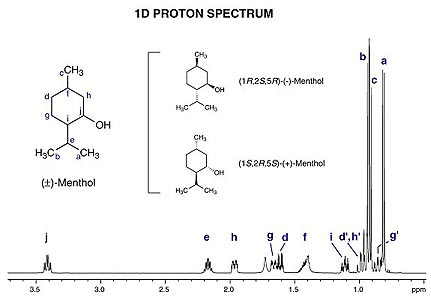
\includegraphics[height=.16\textheight]{files/images/spectrum_nmr_proton_menthol.png}
		\caption{$^{\text{1}}$H NMR spectrum of menthol.}
		\label{SpectrumNmrMenthol}
	\end{minipage}
	}
	\quad
	\fbox{
	\begin{minipage}[b]{0.38\linewidth}
		\centering
		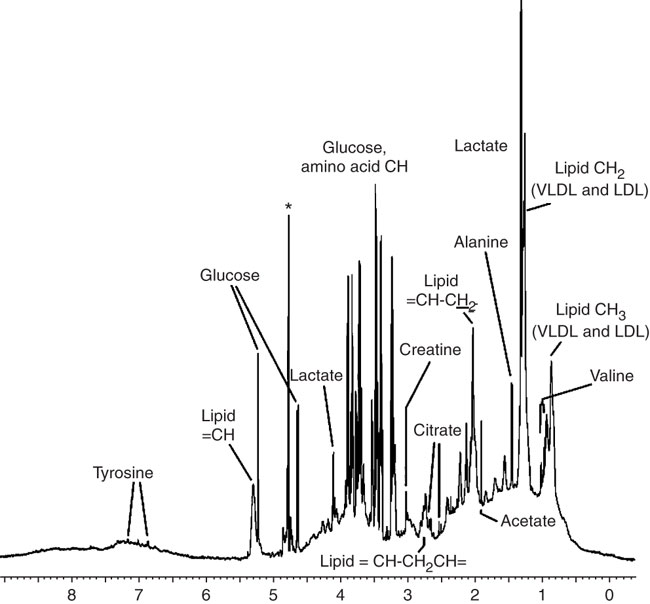
\includegraphics[height=.14\textheight]{files/images/spectrum_nmr_proton_blood.jpg}
		\caption{600 MHz $^{\text{1}}$H NMR spectrum of blood serum sample\protect\footnotemark.}
		\label{SpectrumNmrBlood}
	\end{minipage}
	}
\end{figure}

\footnotetext{source: \url{http://www.nature.com/nprot/journal/v2/n11/fig_tab/nprot.2007.376_F2.html}}


\subsubsection{Data and Metadata}
Metadata or metacontent is data about data. Currently, it is defined as the data providing information about one or more aspects of the data, such as: means of creation data, purpose, creator or standards used \footnote{source: \url{http://en.wikipedia.org/wiki/Metadata}}.
In this information system, we are interesting in data and metadata which can provide hight quality informations in spectral comparison, annotations and identification. The large set of features collected should increase the global quality of the database contents. Externals tools used for searching and queriing, need compound and spectral data and also metadata.\\

This schema represents the different spectrum types and their properties:


\begin{figure}[htbp]
	\centering
	\fbox{
		\begin{minipage}{11 cm}
			\centering
			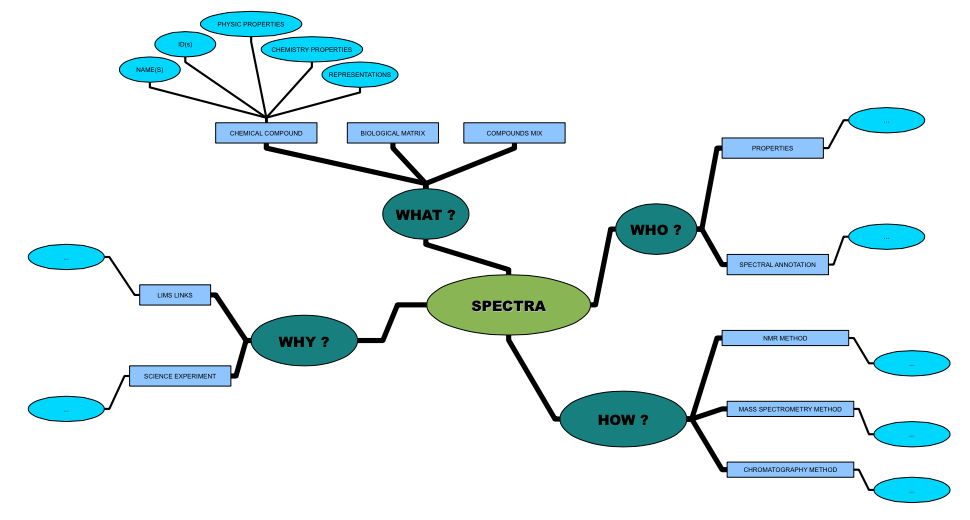
\includegraphics[height=.24\textheight,page=1]{files/images/peakforest_spectrum_types.png}
			\caption{PeakForest -  Initial spectral types }
			\label{PeakForestInitSpectralTypes}
		\end{minipage}
	}
\end{figure}

Regarding the information complexity, the PeakForest data model integrates four levels such as sample, chromatography, spectrum and owner data.


\subsubsection{A user}
According to MetaboHub consortium rules, PeakForest access and consultation require an authentication. Each users should be recorded in the system through an "identifiant user name" and a password. A group of administrators will be in charge of user registration, account creation and role assignment.


%%%%%%%%%%%%%%%%%%%%%%%%%%%%%%%%%%%%%%%%%%%%%%%%%%%%%%%%
%% 						TECHNICAL SPEC
%%%%%%%%%%%%%%%%%%%%%%%%%%%%%%%%%%%%%%%%%%%%%%%%%%%%%%%%

\section{Technical specifications}

\subsection{Teams involved}

The PeakForest project involves the four MetaboHub teams with different roles and resources:
\begin{itemize}
	\item INRA, UMR 1019, PFEM, Clermont-Ferrand  - Project management, machine design, core application and webApp design and building 
	\item CEA, LIST, Laboratory for Data Analysis and Smart Systems (LADIS),  Saclay - MS expertise, peak matching algorithm.
	\item INRA, Metabolome Facility of Bordeaux Functional Genomics Center, Bordeaux - NMR expertise, peak matching algorithm.
	\item INRA, UMR 1331, PF MetaToul-AXIOM, Toxalim, Toulouse - - MS/NMR expertise
\end{itemize}

The product should delivered at the end of the year 2015. The following table present resource repartition and availability.
\begin{figure}[htbp]
	\centering
	\fbox{
		\begin{minipage}{14 cm}
			\centering
			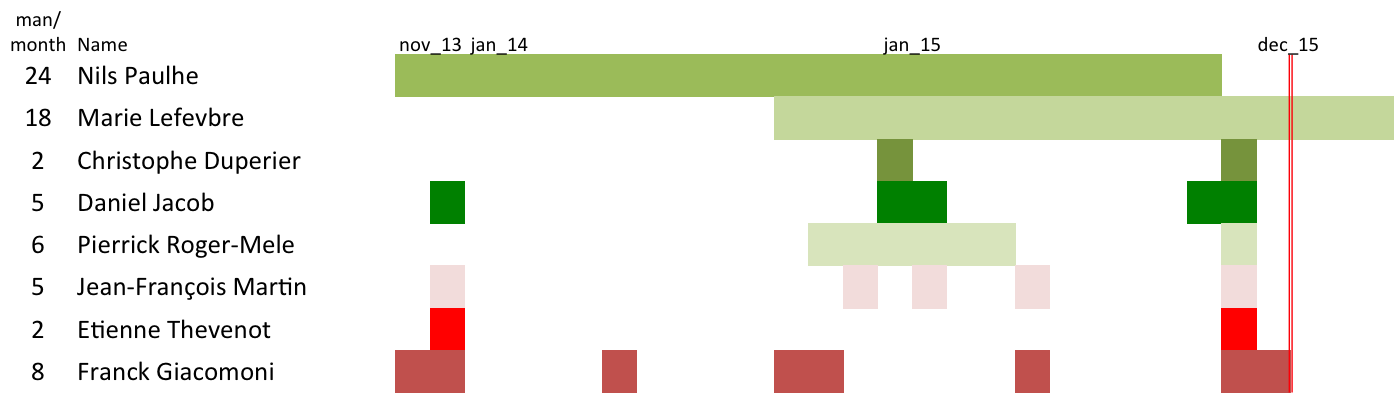
\includegraphics[height=.15\textheight,page=1]{files/images/peakforest_teams_agenda.png}
			\caption{PeakForest -  Resources repartition during the projet }
			\label{PeakForestCompoundObject}
		\end{minipage}
	}
\end{figure}


\subsection{Applicative environment and hardware}

PeakForest is a classical web application using a computer programming language, class-based and object-oriented with model–view–controller software architectural pattern for implementing user interfaces, a database engine for data storage and a web server to be consulted.


\subsubsection{Client environment}

The client must have an internet connection or an intranet network access with a local instance of the software. We recommend a minimum bandwidth of 1.5 Mbps down / 128 Kbps up speed (DSL or fibre connection) to correctly interact with the web-portal. Users view data displayed on their \textbf{screen} and submit request through their \textbf{keyboad} and \textbf{mouse}.
We advice to the clients to use an up-to-date web-browser compliant with W3C standards\footnote{World Wide Web Consortium website: \url{http://www.w3.org/TR/}}. We assume that client computer gets \textbf{2 GB memory or more} to ensure a high quality navigation.\\


\subsubsection{PeakForest hardware}

The PeakForest application will be deploy on a dedicated virtual machine hosting on a platform virtualization. To manage the infrastructure, a virtual machine manager like VMWare is recommended. The figure \ref{performanceRequirement} describe the minimal and recommend hardware requirement for the host-server.

\begin{figure}[htbp]
	\centering
	\fbox{
		\begin{minipage}{16 cm}
		\centering
		\bgroup
		\def\arraystretch{1.3}
		\begin{tabular}{ l l l } 
			\space & Minimal & Recommended \\ 
			Processor & 2 Ghz & $\geq$ 2.4 Ghz \\ 
			Processors number & 2 & $\geq$ 4 \\ 
			Memory & 16 GB & $\geq$ 32 GB \\ 
			Disk space & 50 GB & $\geq$ 1 TB \\ 
%			JRE & v1.7+ & v1.7+ \\
%			Tomcat & 6 & 7+ \\
		\end{tabular} 
		\egroup
		\caption{Performance requirement}
		\label{performanceRequirement}
		\end{minipage}
	}
\end{figure}

A build of a virtual machine template will be proposed to ensure the collaborative part of the project and the portability of the application. Its include all libraries, dependancies and third-part softwares required.


\subsubsection{Server architecture}

The proposed operating system should be a up-to-date server version, with robust and large choices of dependance packages. A Linux CentOS or Ubuntu distribution combines these  properties and The Clermont-Ferrand team has managing experience on such configuration type. 

The use of Java (version 7.x) requires deployment of Java Runtime Environment (JRE version 1.7+) and a compliant Java server (Tomcat 7.x).
All data and data model will use a database engine like MySQL (version 5.x) or PostGreSQL (version 9.x) or MariaDB (version 10.x).


\subsubsection{External dependencies}

Several tools and web services allow {\itshape in silico} operations on chemical compound and spectra. The following list present  the well known and most used tool in laboratories.

\begin{description}
	\item [OpenBabel:]  A chemical toolbox designed to  search, convert, analyze, or store data from molecular modeling, chemistry, solid-state materials, biochemistry, or related areas - Open and collaborative project.
	\item [KeGG compound:] A collection of small molecules, biopolymers, and other chemical substances that are relevant to biological systems. KEGG web services allow customization of KEGG-based analysis - Limitation at an academic use by academic users belonging to academic institutions.
	\item [PubChem:] Three linked databases within the NCBI's Entrez information retrieval system (PubChem Substance, PubChem Compound, and PubChem BioAssay). WebServices allow specialized search and analysis services,  chemical structure searches and full record downloads - American project (NCBI)
	\item [Chemical Entities of Biological Interest  (chEBI):] A freely available dictionary of molecular entities focused on small chemical compounds. ChEBI web services allow programmatic access to the ChEBI database - European project (EBI).
	\item [ChemSpider:] A free chemical structure database providing text and structure search access (Web services) to over millions structures from hundreds of data sources.- Require a personal registration token.
\end{description}

These solutions are integrated and available in PeakForest.


\subsubsection{Hosting, availability and maintenance}

The server and its application are hosting at Clermont Ferrand, at INRA Center. MetaboHub is asking a agreement with the DSI team in charge of INRA data centers exploitation.\\

Monthly scheduled maintenances with service interruptions are required to manage server security releases and server physical resources. The administrator team should reach a goal of a 97\% service availability which represent a downtime duration of 10.96 days per year or 21.6 hours per months or 5.04 hours per week.\\
 
Administrators are in charge of PeakForest software updates deployment. They are checking physical resources (processors / memory / disk space / bandwidth) required by the software on the server and its uptime.


\subsubsection{Security}
A dedicate server is hosting PeakForest software and database. The server is opened to internet and placed into a dedicated subnetwork (demilitarized zone). Supplementary security packages like Fail2Ban or IpTables are also expected. \\

The version of PeakForest delivered for the MetaboHUB consortium is integrating the "Lightweight Directory Access Protocol" (LDAP) authentications system using at INRA.


\subsection{Product specifications}

The back-end execution core is based on the JAVA language. The front-end part of the project will be written under HTML5, a descriptive language and Javascript, a programming language. Peak matching algorithms should be written in R and Python.


\subsubsection{Product functions}

\begin{itemize}
	\item Users: save / edit / delete / find Spectra in the database; check if a user is allowed to perform an operation.
	\item Chemical Compounds: save / edit / delete / find Spectra in the database.
	\item Spectra: save / edit / delete / find Spectra in the database.
	\item Annotation process: use stored data an knowledge to provide a computer assistance for Spectra annotation.
\end{itemize}


\subsubsection{System interfaces}

The PeakForest core is developed as an API which offer the possibility to implement several services and interfaces. With PeakForest, the API is used by the web-portal (web application) and called through web services. The main access  is though public web-portal, providing several interfaces depending on the user certification level (\cf section \ref{userInterfaces} page \pageref{userInterfaces}).

Third-party software or script access to the spectral database via these webservices. The R.E.S.T\footnote{For informations please refer to this \href{https://www.ics.uci.edu/~fielding/pubs/dissertation/rest_arch_style.htm}{introduction} about Representational State Transfer.} protocol is recommended with the support of both POST and GET methods and JSON\footnote{Official specifications: \url{http://json.org/}} objects returns. This sort of interface provide tools to get PeakForest data but none consulting or editing operations. 

\begin{figure}[htbp]
	\centering
	\fbox{
		\begin{minipage}{12 cm}
			\centering
			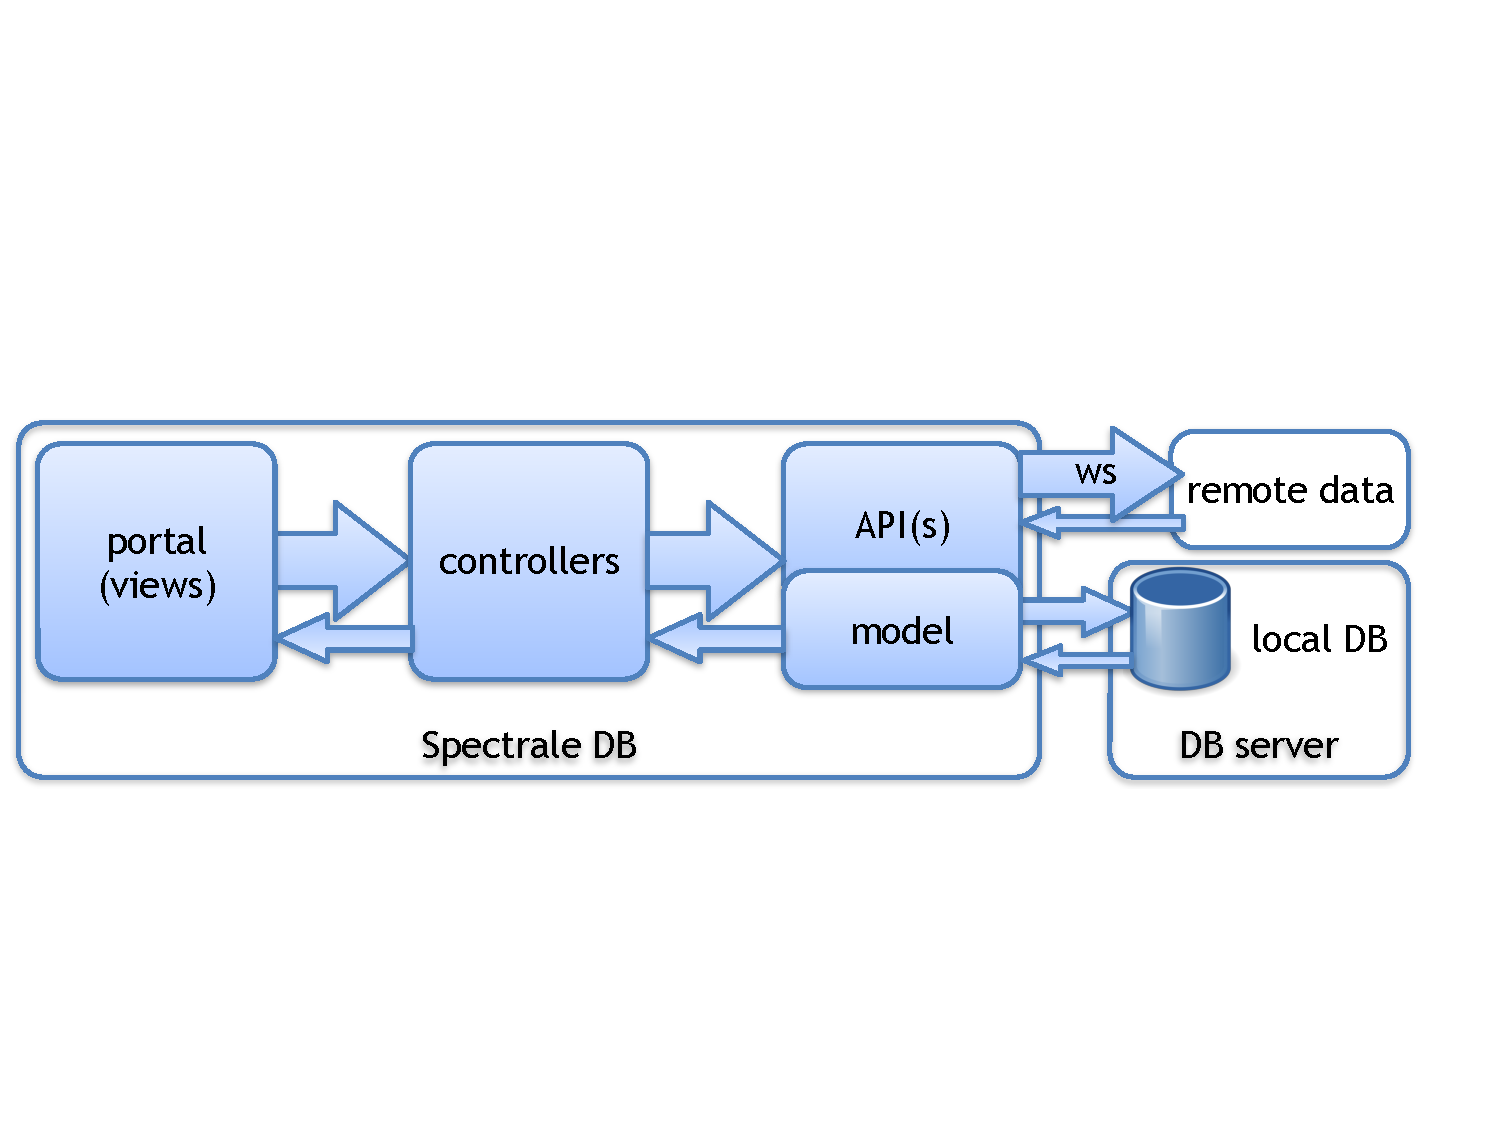
\includegraphics[height=.13\textheight,page=1]{files/pdf/mvc1.pdf}
			\caption{Software Architecture (1/2): Web portal}
			\label{SoftArchi1}
		\end{minipage}
	}
	\quad
	\centering
	\fbox{
		\begin{minipage}{12 cm}
			\centering
			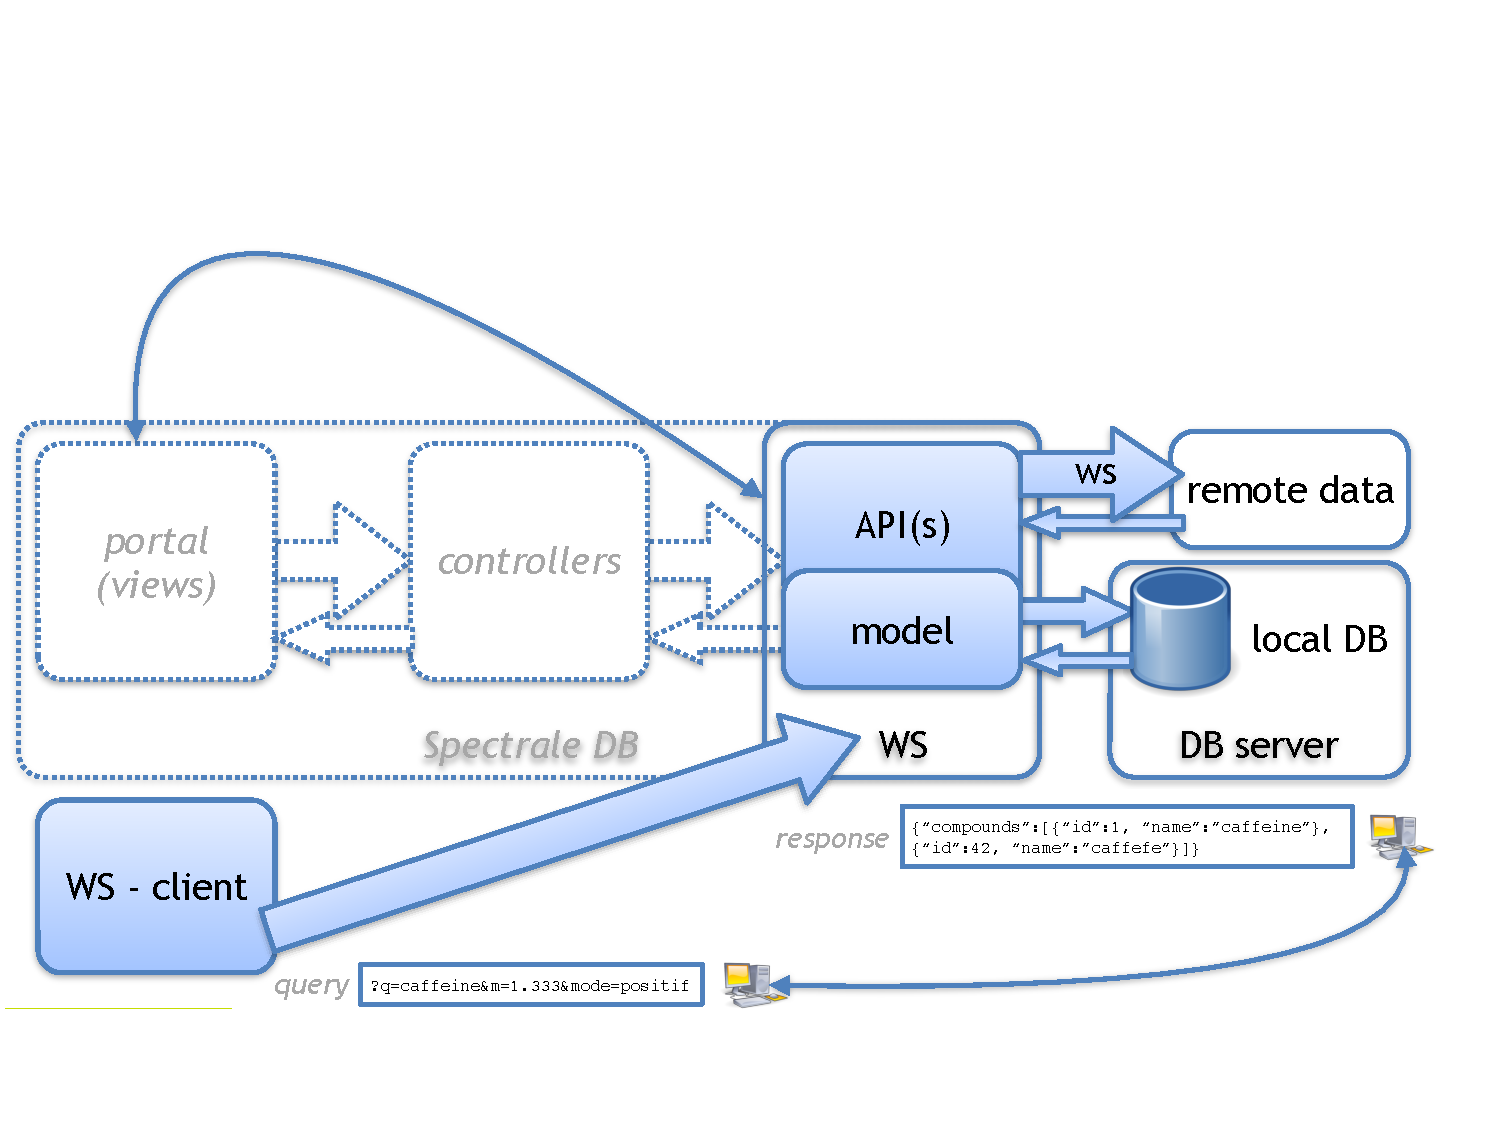
\includegraphics[height=.24\textheight,page=1]{files/pdf/mvc2.pdf}
			\caption{Software Architecture (2/2): Web ervices}
			\label{SoftArchi2}
		\end{minipage}
	}
\end{figure}

The figures \ref{SoftArchi1} and \ref{SoftArchi2} show how the web-portal and web services use the same API core. 
For security and privacy reasons, the user management service is only implemented on the web-portal side.

PeakForest services are splited into several and distinct API (\cf figure \ref{SoftArchi3}). This architecture facilitate the re-use of some core functionalities, releases of files parsers and the adaptability to externals resources and tools.

\begin{figure}[htbp]
	\centering
	\fbox{
		\begin{minipage}{12 cm}
			\centering
			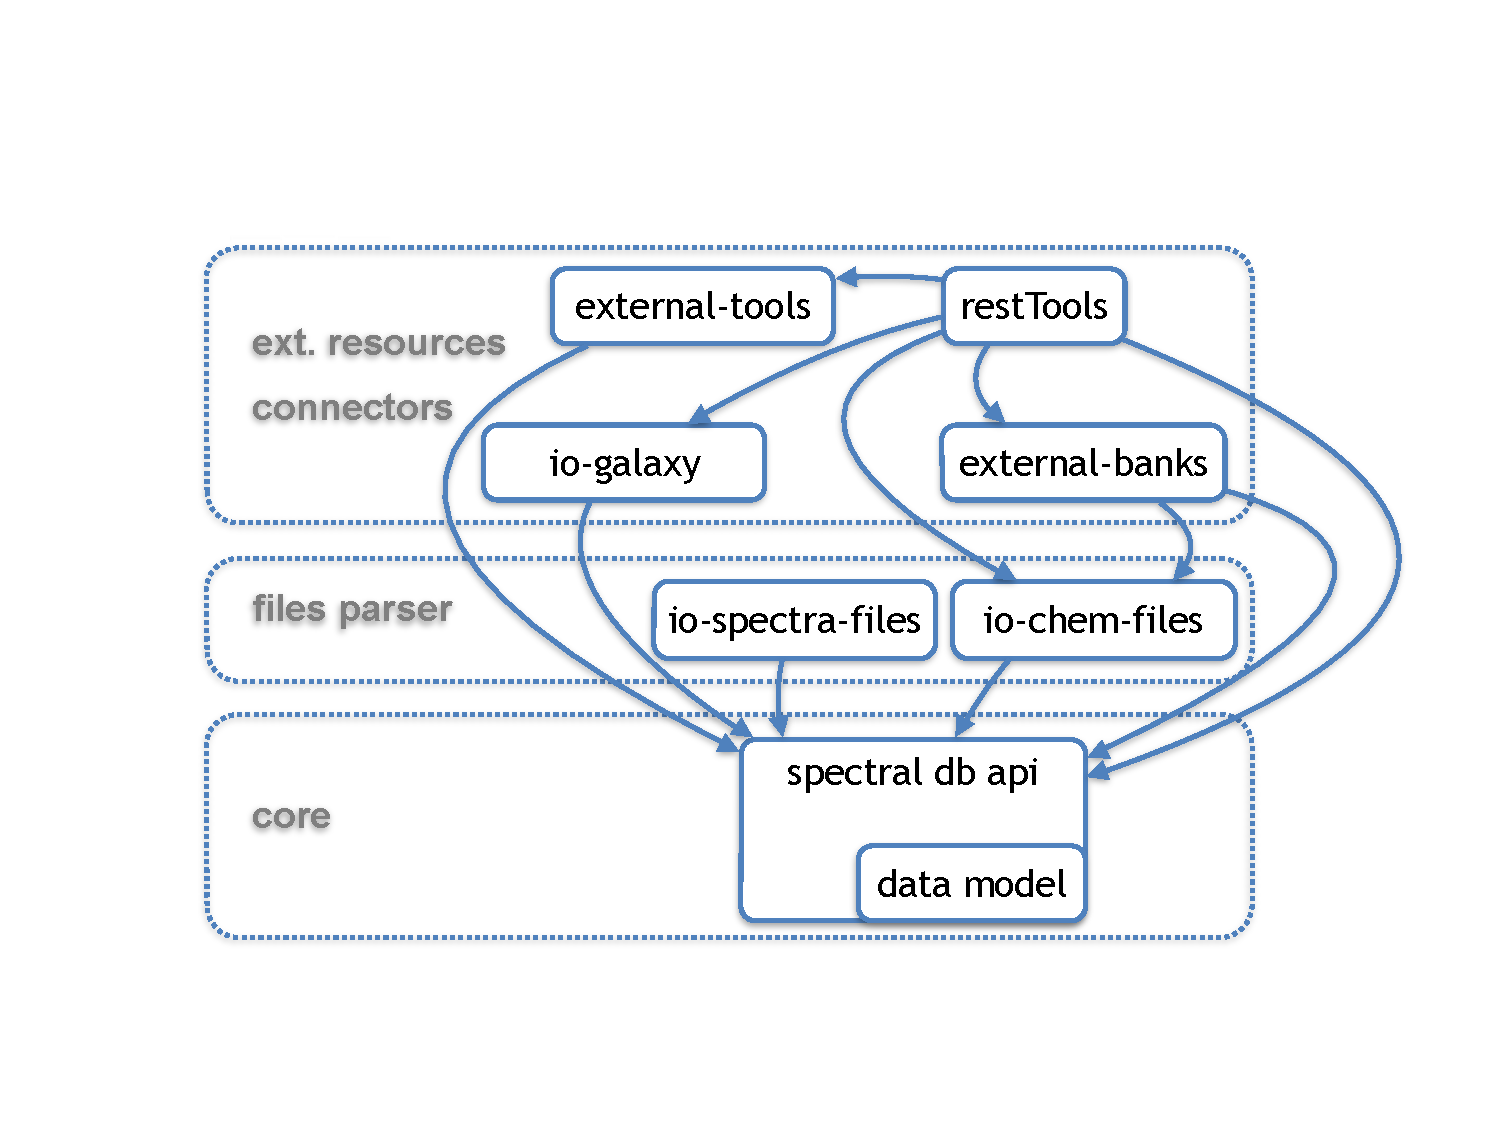
\includegraphics[height=.24\textheight,page=1]{files/pdf/api.pdf}
			\caption{API interactions and encapsulations}
			\label{SoftArchi3}
		\end{minipage}
	}
\end{figure}

\subsubsection{User roles}

To manage PeakForest web portal access, a user authentication system is implemented. A non-registered user will only be able to see data in public databases. He need to sign-up or register. The account validation process require an administrator authority. 
An user has rights defined by a role assigned after validation by an administrator.\\

A \textbf{validated user} is allow to add new data in the public database or in the group shared databases, annotate spectra and report error or missing informations in the database. It can not edit textual data but can suggest modifications through curation messages associated with different objects (compound or spectra).\\

An administrator has the opportunity to promote a user as \textbf{curator}. The curator role permit textual data edition via the curation messages center. Finally, an user can become an administrator or lost its granted rights.\\

An \textbf{administrator} is in charge of performing maintenance jobs. He accumulate validated user and curator rights.\\

%Once converted into group, a user can not add new or edit data in public / group shared database; 
%if it is used to have a group shared database, it loses the right to interact with them. 
%It adds add / remove "normal" users (with approved, curator or admin rights), inviting them to interact with a database created for this group and shared with any user belonging to the group.
%A user can belong to more than one group (it has to select the public or a group-shared database first, then it cannot interact with data in other database).
%If a user is not in a group, it can only interact with the public database.

The following figure resume rights and roles of users in PeakForest web-portal :

\begin{figure}[htbp]
	\centering
	\fbox{
		\begin{minipage}{16 cm}
			\centering
			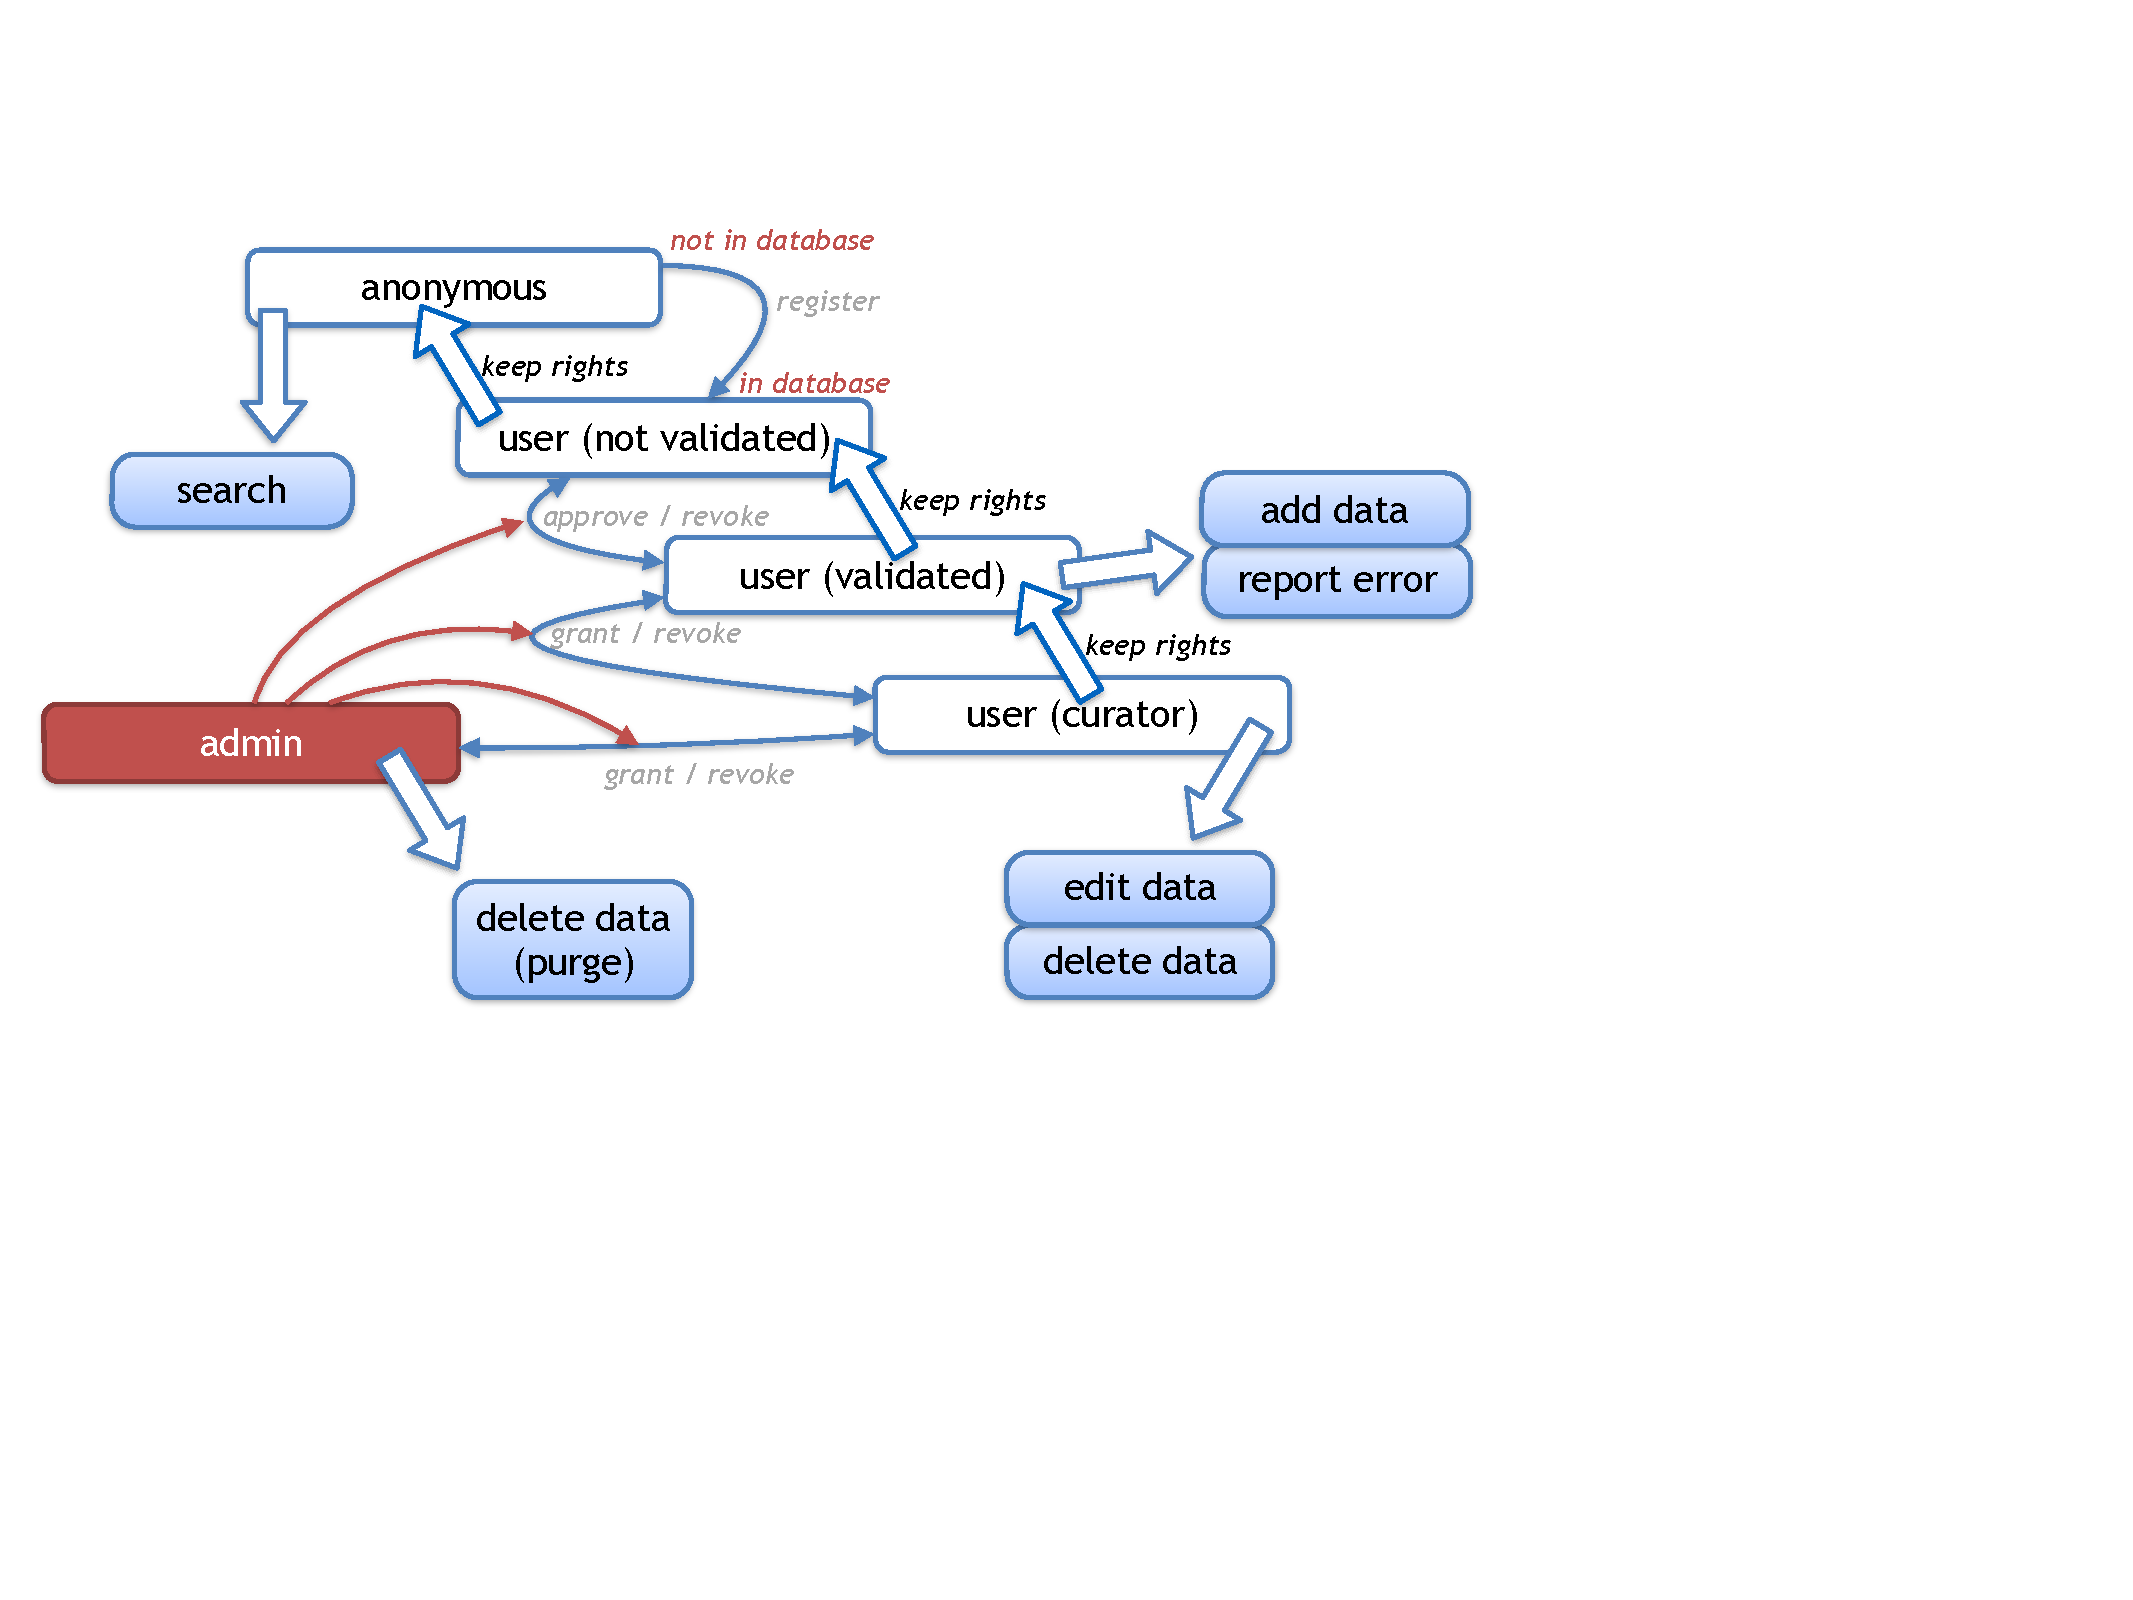
\includegraphics[height=.26\textheight,page=1]{files/pdf/users_rights.pdf}
			\caption{User rights}
			\label{userRights}
		\end{minipage}
	}
\end{figure}

\subsubsection{Operations}

\textbf{User management (all GUI only):}
\begin{itemize}
	\item Request an account.
	\item Validate an account.
	\item Promote / demote user rights (user / curator / administrator).
	\item Convert user to group.
	\item Invite user / revoke user invitation to a group.
\end{itemize}
~\\
\textbf{Chemical Compounds management:}
\begin{itemize}
	\item Perform global search on chemical compound library (GUI + WS).
	\item Get all data on a chemical compound (GUI + WS).
	\item Add a single chemical compound (GUI).
	\item Add a list of chemical compounds (from template file) (GUI).
	\item Edit chemical compound informations (GUI).
	\item Delete a single chemical ompound (GUI).
	\item Perform clean jobs on chemical compound library (GUI).
\end{itemize}
~\\
\textbf{Spectra management:}
\begin{itemize}
	\item Perform global search on spectra (GUI + WS).
	\item Get all data on a spectra (GUI + WS).
	\item Add a single spectra; link data / metadata to it (GUI).
	\item Add a list of spectra (from template file); link data / metadata to them (GUI).
	\item Edit a spectra basic informations / metadata (GUI).
	\item Annotate a spectra stored in the database (GUI).
	\item Annotate a spectra on-the-fly (GUI).
	\item Delete a single spectra (GUI).
	\item Perform clean jobs on spectra (GUI).
\end{itemize}
~\\
\textbf{Annotation process:}
\begin{itemize}
	\item Link a spectra with chemical compound(s) (GUI).
	\item Link chemical compounds (reference) to other chemical compounds (putative) (GUI).
	\item Save annotation results for spectra library.
\end{itemize}

\subsubsection{User interfaces} \label{userInterfaces}

Accesses of interfaces depends to the user accreditation level.\\
~\\~
\textbf{Anonymous users / not yet validated users:}
\begin{itemize}
	\item Search / get data on reference chemical compounds in the public library;
	\item Search / get data on spectra in the public database;
	\item Submit "on the flight" annotations queries.
	\item Delete the user account (only for not validated users).
\end{itemize}
~\\
\textbf{Validated users:}
\begin{itemize}
	\item All interfaces described in anonymous users / not yet validated users section.
	\item Add new reference chemical compounds in the public database;
	\item Add new reference chemical compounds in a group shared database;
	\item Add new spectra and their metadata in the public database;
	\item Add new spectra and their metadata in a group shared database;
	\item Annotate spectra;
	\item Convert itself as a group (not reversible);
	\item Add curation messages to several entities.
\end{itemize}
~\\
\textbf{curator users:}
\begin{itemize}
	\item All interfaces described in anonymous users / not validated user section.
	\item All interfaces described in validated users section (not the "convert in a group" and "add curation messages" options!).
	\item Edit reference chemical compounds in a group shared database;
	\item Edit spectra in the public database;
	\item Edit spectra in a group shared database;
	\item Remove curation messages linked entities.
\end{itemize}
~\\
\textbf{Administrators:}
\begin{itemize}
	\item All interfaces described in anonymous users / not validated user section.
	\item All interfaces described in validated users section (not the "convert in a group" and "add curation messages" options!).
	\item All interfaces described in curator users section.
	\item Run bash cleaner job.
	\item Perform maintenance job.
	\item Change users rights (set a different role described in previous sections).
\end{itemize}
~\\
\textbf{Users as a group:}
\begin{itemize}
	\item Invite a user to interact with the group's database.
	\item Reject a user's invitation (revoke his access to the group-shared database linked to the group).
	\item Rename the database link to the group.
\end{itemize}

This case is a special use case, only available for user converted as a group (can not be promote or demote by administrator).


\subsection{Build organisation}

Each team is involved in software building process with different programming languages. 

\subsection{Documentation}
Ergonomics of the website ensure the use of PeakForest and its interface without any formation or documentation reading.
The Spectral Database web-portal and webservices will be delivered with documentation both user and developer instruction manuals: 
the first for all software users, the second only destined to developer / system administrator (with advanced instruction about how to deploy manage and maintain the software / servers).



\subsection{Portability}

Official releases of the software have two principal delivering forms: 
\begin{itemize}
	\item Packaged war file, ready to be deploy on a Java server.
	\item Complete virtual machine with PeakForest software and versionned databases
\end{itemize}




\newpage
\newpage

%%%%%%%%%%%%%%%%%%%%%%%%%%%%%%%%%%%%%%%%%%%%%%%%%%%%%%%%
%% 						APPENDIX
%%%%%%%%%%%%%%%%%%%%%%%%%%%%%%%%%%%%%%%%%%%%%%%%%%%%%%%%

\appendix
\pagenumbering{roman}
\setcounter{page}{1}

\makeatletter
\def\@seccntformat#1{Appendix~\csname the#1\endcsname:\quad}
\makeatother

\section{The PeakForest Data Model View.}
\label{AppendixDataModel}

\begin{figure}[h!]
	\centerline{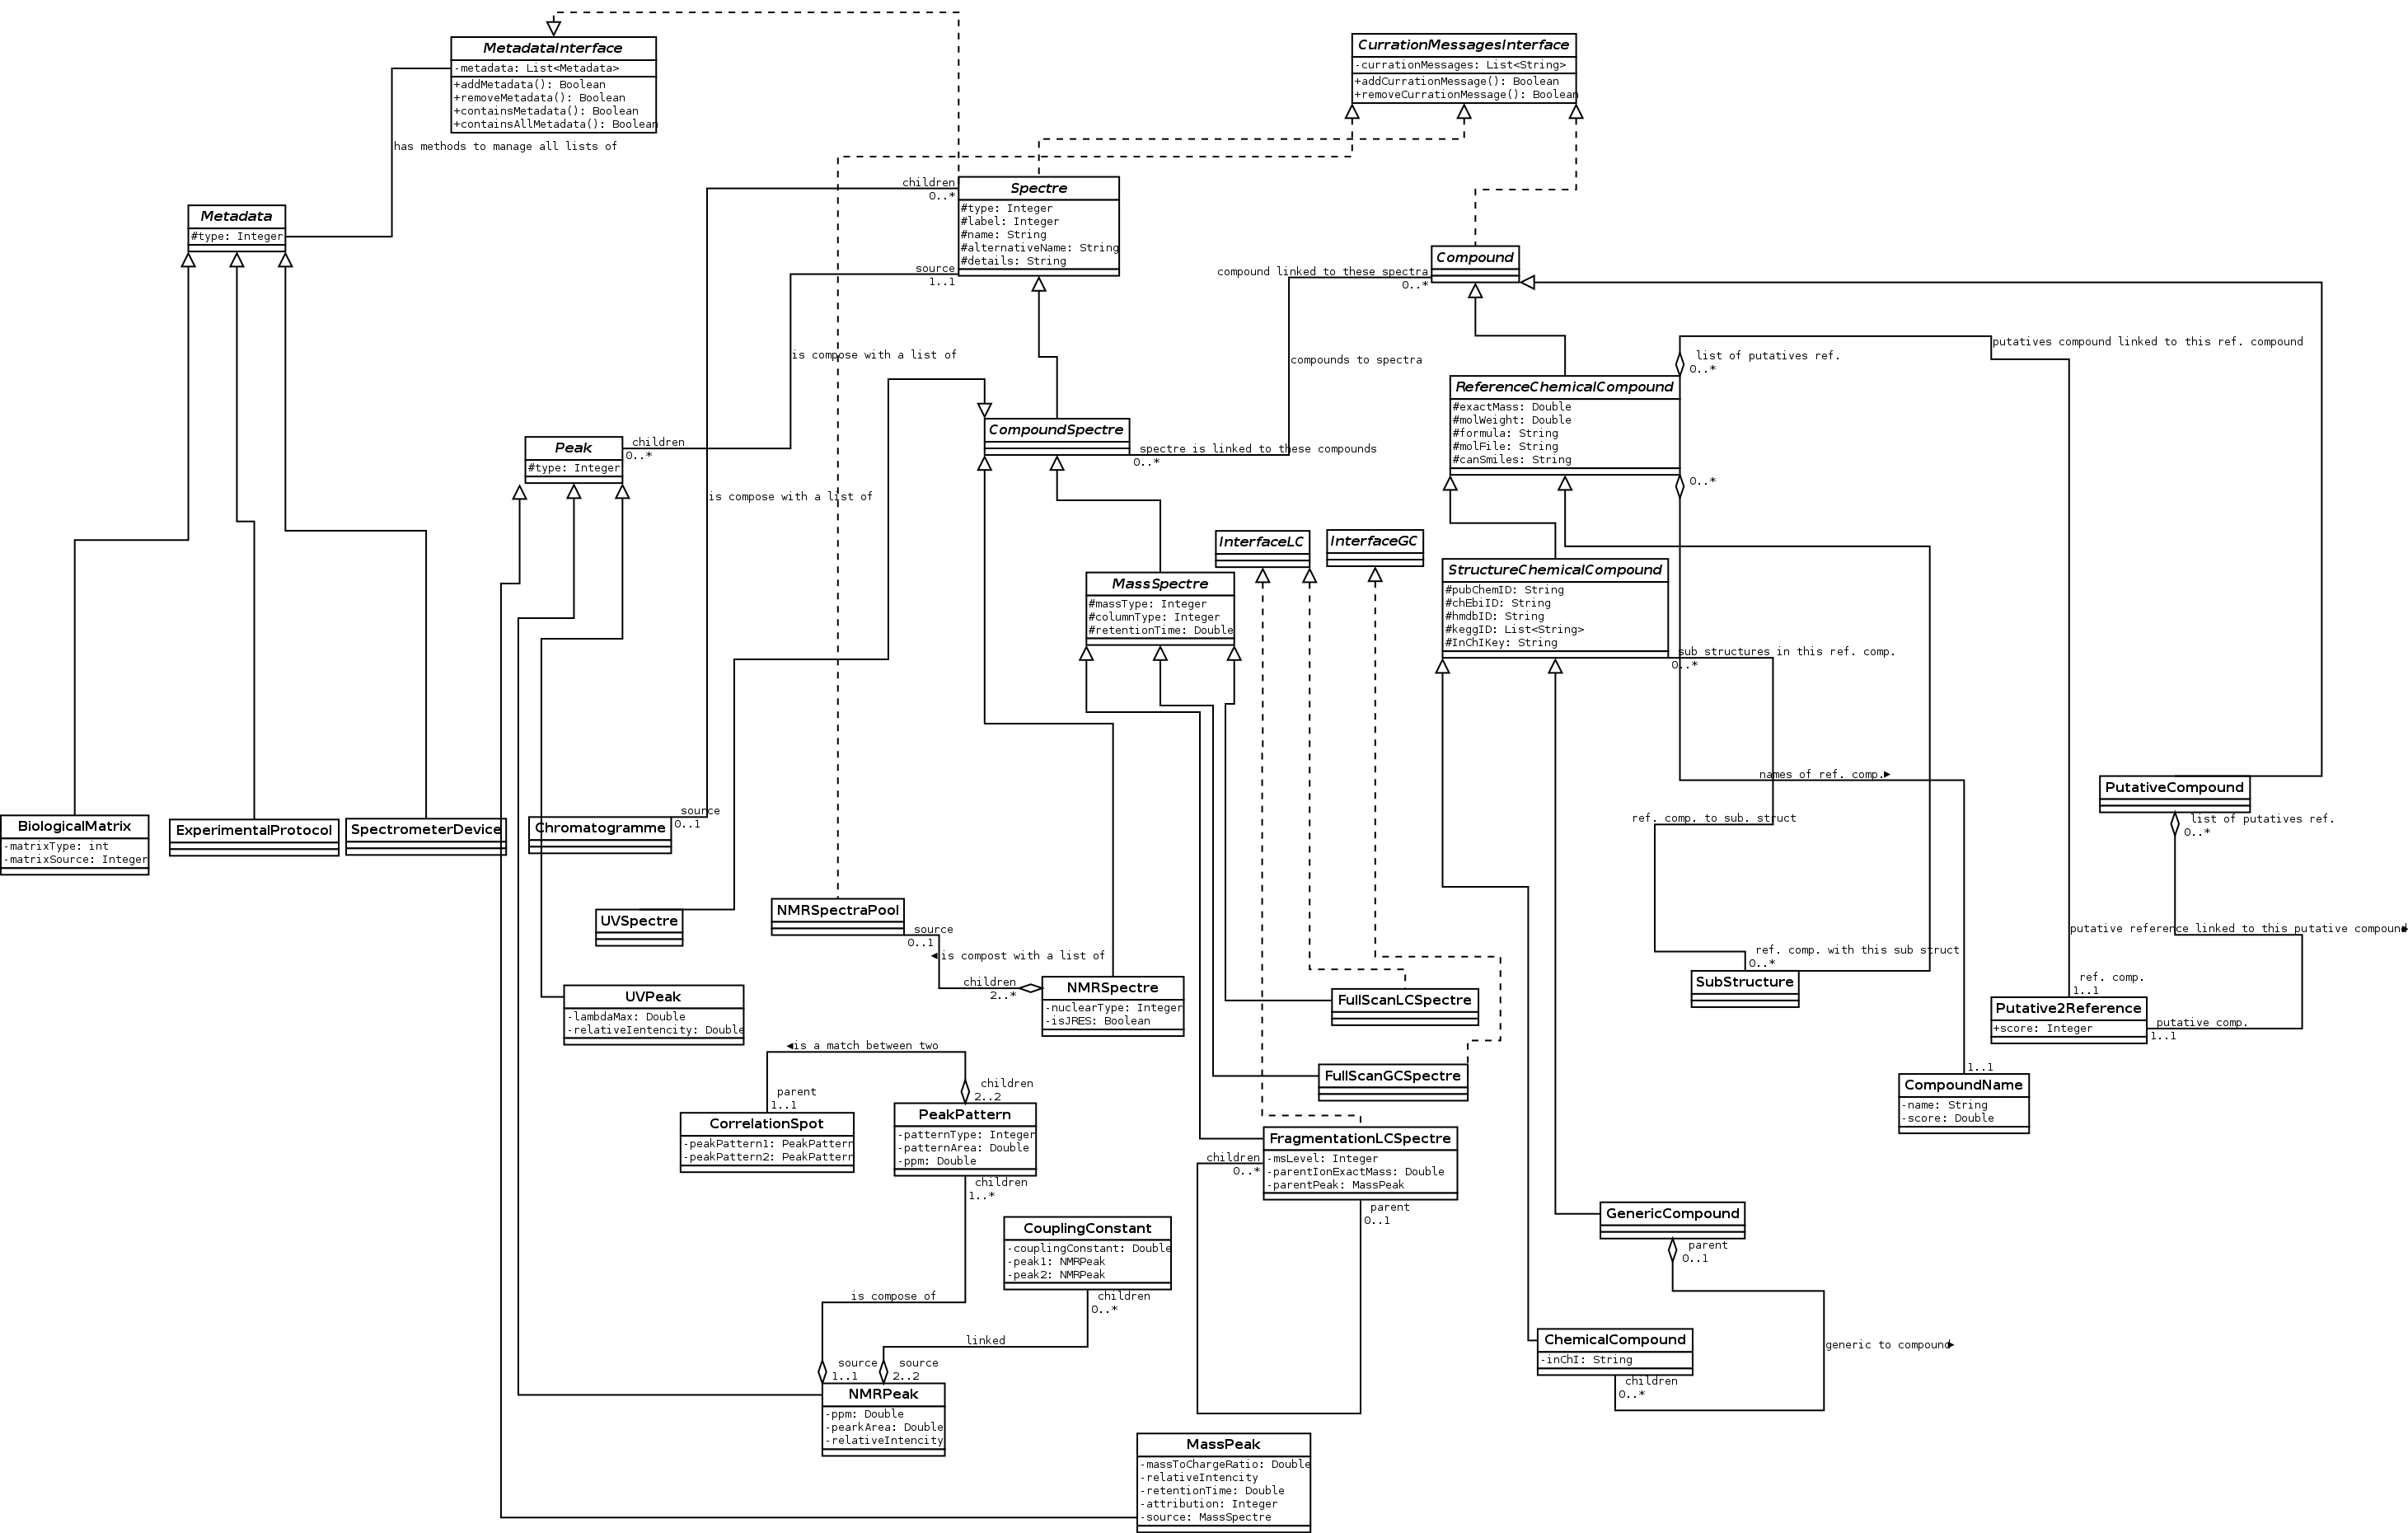
\includegraphics[width=23cm, angle =270]{files/images/peakforest_data-model.png}}
%	\caption{PeakForest Data Model View}
	\label{PeakForestDataModelView}
\end{figure}


\section{User-Interface interaction UML diagrams}
\label{AppendixUMLDia}

The three following diagrams represent the possible interaction between users (chemists) and the PeakForest interfaces. A chemist should search from a chemical compound and a spectrum. 

\begin{figure}[h!]
	\centerline{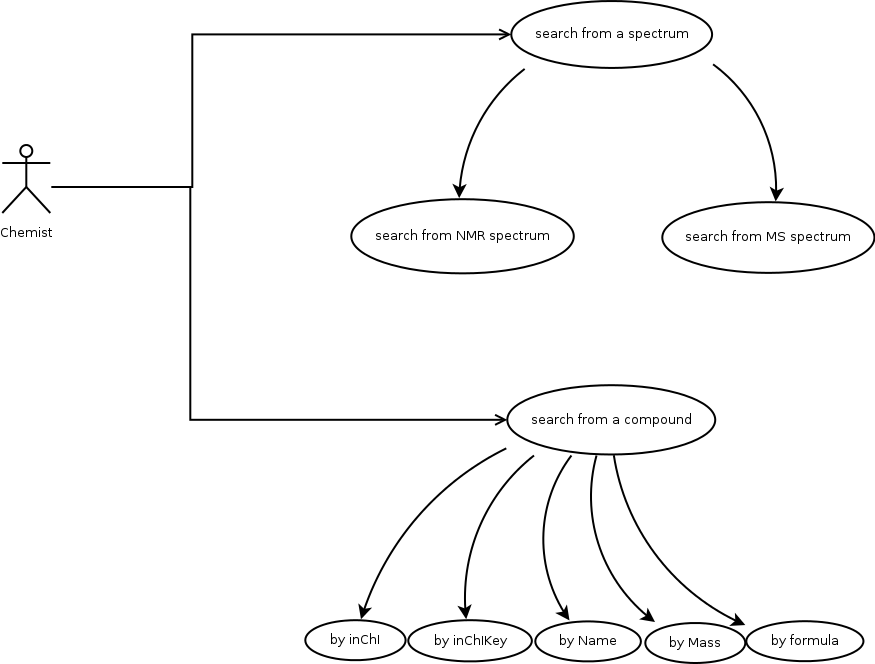
\includegraphics[width=9cm]{files/images/peakforest_gui_uml_searches.png}}
\end{figure}

\begin{figure}[h!]
	\centerline{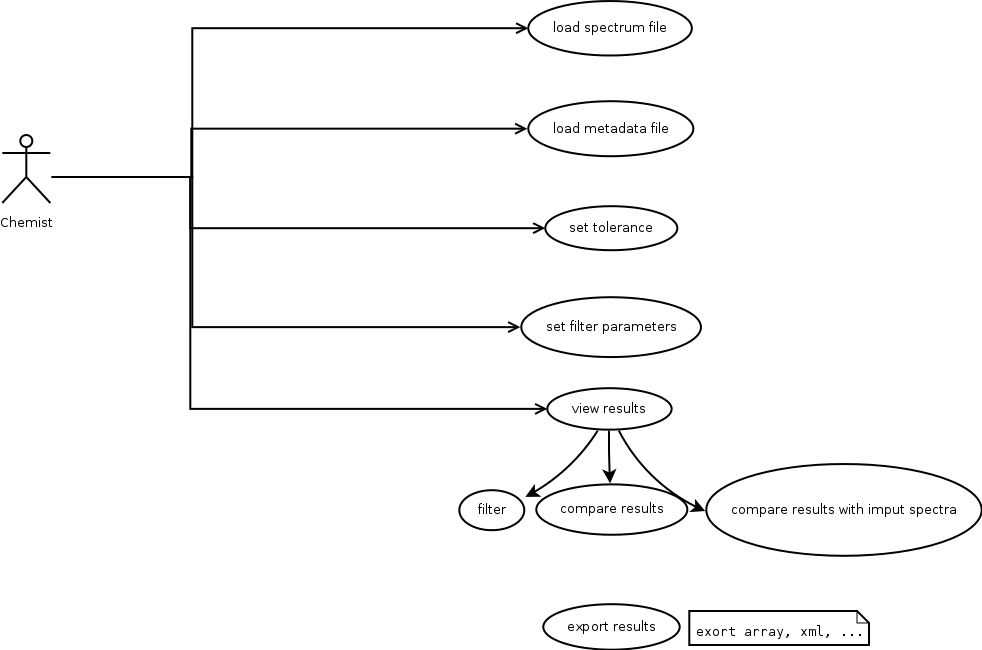
\includegraphics[width=10cm]{files/images/peakforest_gui_uml_search_NMR.png}}
\end{figure}

\begin{figure}[h!]
	\centerline{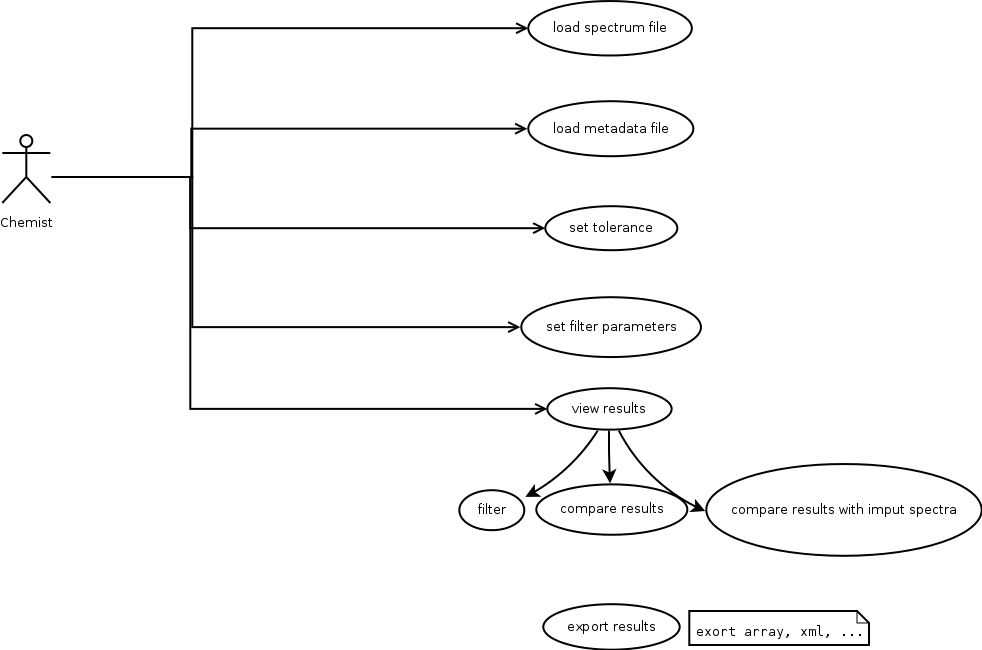
\includegraphics[width=10cm]{files/images/peakforest_gui_uml_search_MS.png}}
\end{figure}




\end{document}